% ============================================================================
%  4. RESULTADOS  (125--165 min)
%  Todas las cifras: regla de decisión de Dynare 7.1 (rbc_analytical.mod) en
%  elasticidades. Notación de la pizarra: \hat k_t es el capital en uso en t.
% ============================================================================
\section{Resultados}

% S33
\begin{frame}[label=receta]{La receta: de dónde sale cada número}
  \begin{columns}[T,onlytextwidth]
    \begin{column}{0.44\textwidth}
      \small
      \textbf{1. El choque}\par
      $\hat a_1=\sigma_\varepsilon=0.72\%$\par
      \vspace{0.25cm}
      \textbf{2. Condición inicial}\par
      $\hat k_1=0$: el capital ya estaba elegido.\par
      \vspace{0.25cm}
      \textbf{3. Los estados avanzan}\par
      $\hat a_{t+1}=0.979\,\hat a_t$\par
      $\hat k_{t+1}=0.936\,\hat k_t+0.125\,\hat a_t$\par
      \vspace{0.25cm}
      \textbf{4. Cada variable}\par
      $\hat x_t=\eta_{xk}\,\hat k_t+\eta_{xa}\,\hat a_t$
    \end{column}
    \begin{column}{0.52\textwidth}
      \centering\small
      \renewcommand{\arraystretch}{1.2}
      \begin{tabular}{@{}lrr@{}}
        \toprule
        & $\eta_{xk}$ & $\eta_{xa}$\\
        \midrule
        Producto $\hat y$ & 0.108 & 1.477\\
        Consumo $\hat c$ & 0.530 & 0.583\\
        Inversión $\hat\imath$ & $-1.560$ & 5.016\\
        Horas $\hat h$ & $-0.337$ & 0.716\\
        Salario $\hat w$ & 0.445 & 0.762\\
        Alquiler $\hat r$ & $-0.892$ & 1.477\\
        Capital $\hat k_{t+1}$ & 0.936 & 0.125\\
        \bottomrule
      \end{tabular}
    \end{column}
  \end{columns}
  \fuente{Regla de decisión de Dynare pasada a elasticidades, $\delta=0.025$.}
  \note{Las elasticidades salen del control 3: coeficiente en niveles por
  (estado)\_ss/x\_ss. Coinciden con las fórmulas de la PD06, F.5.}
\end{frame}

% S34
\begin{frame}[fragile,label=dynare-confirma]{Dynare da lo mismo, trimestre a trimestre}
  \begin{lstlisting}[language={}]
>> 100*oo_.irfs.y_eps(1:3)/oo_.steady_state(1)
    1.0636    1.0511    1.0381
>> 100*oo_.irfs.c_eps(1:3)/oo_.steady_state(2)
    0.4196    0.4586    0.4938
\end{lstlisting}
  \vspace{0.2cm}
  \texttt{oo\_.irfs} guarda 40 valores por variable, en niveles: se dividen por el
  estado estacionario para pasar a porcentaje.\par
  \vspace{0.25cm}
  El primer elemento es el trimestre del choque.\par
  \vspace{0.25cm}
  Cuidado: el \texttt{k} de Dynare es el capital \emph{elegido}. Su primer valor,
  $0.0903\%$, es el $\hat k_2$ de la pizarra.
  \note{Para la receta: y = 1.477 x 0.72 = 1.064; c = 0.583 x 0.72 = 0.420.}
\end{frame}

% S35
\begin{frame}[label=dos-ideas]{Dos ideas que ordenan la historia}
  \begin{columns}[T,onlytextwidth]
    \begin{column}{0.47\textwidth}
      \textbf{1. El choque es transitorio, aunque persistente}\par
      \vspace{0.25cm}
      $\hat a_t=0.72\times0.979^{\,t-1}$\par
      \vspace{0.2cm}
      Vida media: $\ln 0.5/\ln 0.979\approx33$ trimestres.\par
      \vspace{0.2cm}
      El hogar sabe que la productividad alta no va a durar.
    \end{column}
    \begin{column}{0.47\textwidth}
      \textbf{2. El hogar solo decide dos cosas}\par
      \vspace{0.25cm}
      Cuánto trabajar ($\hat h$) y cómo repartir su ingreso entre consumir ($\hat c$) y
      ahorrar ($\hat\imath$).\par
      \vspace{0.2cm}
      Lo demás son precios que vacían mercados ($\hat w$, $\hat r$) o contabilidad
      ($\hat k$).
    \end{column}
  \end{columns}
\end{frame}

% S36
\begin{frame}[label=acto1]{Acto 1: la foto del impacto, $t=1$}
  \centering\small
  \renewcommand{\arraystretch}{1.2}
  \begin{tabular}{@{}llrl@{}}
    \toprule
    & \textbf{Cálculo} & \textbf{\%} & \textbf{Lectura}\\
    \midrule
    $\hat a$ & choque & 0.720 & la productividad sube\\
    $\hat k$ & predeterminado & 0 & el capital aún no cambia\\
    $\hat y$ & $1.477\times0.72$ & 1.064 & sube más que $\hat a$\\
    $\hat c$ & $0.583\times0.72$ & 0.420 & el consumo sube poco\\
    $\hat\imath$ & $5.016\times0.72$ & \num{3.611} & la inversión se dispara\\
    $\hat h$ & $0.716\times0.72$ & 0.515 & se trabaja más\\
    $\hat w$ & $0.762\times0.72$ & 0.548 & el salario sube\\
    $\hat r$ & $1.477\times0.72$ & 1.064 & el capital rinde más\\
    \bottomrule
  \end{tabular}
  \par\vspace{0.3cm}\raggedright\normalsize
  ¿Quién acertó la votación del inicio sobre las horas?
  \note{Volver a la votación de la slide pregunta. Cifras redondeadas a tres decimales.}
\end{frame}

% S37
\begin{frame}[label=acto1-horas]{Las horas suben porque el consumo sube poco}
  Igualando oferta y demanda de trabajo, con $\hat k_1=0$:
  \[
  \hat h_t=\frac{\hat a_t+(1-\alpha)\hat k_t-\hat c_t}{1-\alpha+\frac{h_{ss}}{1-h_{ss}}}
  =1.7153\times(0.7200-0.4196)=\num{0.5152}
  \]
  \par\vspace{0.1cm}
  El mercado vacía al mismo salario:\par
  \vspace{0.1cm}
  \hspace*{0.4cm}Oferta: $\hat w=\hat c+0.25\,\hat h=0.4196+0.1288=0.5484$\par
  \hspace*{0.4cm}Demanda: $\hat w=\hat y-\hat h=1.0636-0.5152=0.5484$\par
  \vspace{0.3cm}
  El salario sube mucho; la riqueza, poco, porque el choque es transitorio. El
  \textbf{efecto sustitución} (trabajar ahora rinde más) domina al \textbf{efecto
  ingreso} (más rico, más ocio).
  \fuente{$0.25=h_{ss}/(1-h_{ss})$. $1.7153=1/(1-\alpha+0.25)$.}
  \note{Sustitución intertemporal del trabajo: se trabaja más mientras la
  productividad está alta.}
\end{frame}

% S38
\begin{frame}[label=acto1-producto]{Un tercio del producto extra viene de trabajar más}
  Producción log-lineal en $t=1$:
  \begin{align*}
  \hat y_1&=\hat a_1+(1-\alpha)\hat k_1+\alpha\hat h_1\\
  &=0.720+0.333\times0+0.667\times0.515=\num{1.064}
  \end{align*}
  \par\vspace{0.2cm}
  \centering
  \begin{tikzpicture}[scale=0.9, transform shape]
    \fill[darkblue] (0,0) rectangle (6.8,0.55);
    \fill[errframe] (6.8,0) rectangle (10.05,0.55);
    \node[white, font=\small\bfseries] at (3.4,0.275) {productividad: 0.720 (68\%)};
    \node[white, font=\small\bfseries] at (8.42,0.275) {horas: 0.344 (32\%)};
  \end{tikzpicture}
  \par\vspace{0.35cm}\raggedright
  Si las horas no se movieran, el producto subiría $0.72\%$. Con horas sube
  $1.064/0.720=1.48$ veces el choque: la \textbf{amplificación}.
\end{frame}

% S39
\begin{frame}[label=acto1-reparto]{Casi el 70\% del producto extra se invierte}
  Vaciado de bienes, con $s_c=0.798$ y $s_i=0.202$:
  \begin{align*}
  \hat y_1&=s_c\,\hat c_1+s_i\,\hat\imath_1
  =0.798\times0.420+0.202\times3.611\\
  &=0.335+0.729=\num{1.064}
  \end{align*}
  \par\vspace{0.2cm}
  \centering
  \begin{tikzpicture}[scale=0.9, transform shape]
    \fill[UWGrayL3] (0,0) rectangle (3.17,0.55);
    \fill[tipframe] (3.17,0) rectangle (10.05,0.55);
    \node[white, font=\small\bfseries] at (1.58,0.275) {consumo 31\%};
    \node[white, font=\small\bfseries] at (6.61,0.275) {inversión 69\%};
  \end{tikzpicture}
  \par\vspace{0.35cm}\raggedright
  \textbf{Suavizamiento}: el hogar sabe que el choque pasará y ahorra la mayor parte del
  ingreso extra.\par
  \vspace{0.2cm}
  Además, ahorrar paga más: $\hat r_1=\hat y_1-\hat k_1=1.064$.
\end{frame}

% S40
\begin{frame}[label=acto2-capital]{Acto 2: el capital se acumula despacio}
  Ley de movimiento:\quad $\hat k_{t+1}=(1-\delta)\,\hat k_t+\delta\,\hat\imath_t$
  \vspace{0.15cm}
  \begin{align*}
    \hat k_2&=0.975\times0+0.025\times3.611=0.090\\
    \hat k_3&=0.975\times0.090+0.025\times3.395=0.173
  \end{align*}
  Reordenando: $\hat k_{t+1}-\hat k_t=\delta\,(\hat\imath_t-\hat k_t)$. El capital crece
  mientras $\hat\imath_t>\hat k_t$.\par
  \vspace{0.3cm}
  En $t=26$: $\hat\imath=0.825<\hat k=0.833$. El capital toca su \textbf{máximo}.\par
  \vspace{0.3cm}
  Una inversión enorme mueve poco un stock grande: esa lentitud es la
  \textbf{propagación interna}.
  \fuente{$\hat\imath_2=3.395=-1.560\times0.090+5.016\times0.705$.}
\end{frame}

% S41
\begin{frame}[label=acto2-consumo]{El consumo sube mientras el capital rinda de más}
  Euler. Sin nuevos choques, lo esperado es lo que ocurre:
  \[
  \hat c_{t+1}-\hat c_t=\beta r_{ss}\,\hat r_{t+1},\qquad \beta r_{ss}=0.0406
  \]
  \par\vspace{0.1cm}
  $t=1$:\quad $\hat c_2-\hat c_1=0.459-0.420=0.039=0.0406\times0.961$\par
  \vspace{0.3cm}
  \begin{tabular}{@{}ll@{}}
    $\hat r_{19}=+0.017$ & el consumo todavía sube\\
    $\hat r_{20}=-0.008$ & empieza a bajar
  \end{tabular}
  \par\vspace{0.3cm}
  El consumo tiene forma de \textbf{joroba}: su máximo, $0.707\%$, está en $t=19$,
  justo antes de que $\hat r$ se vuelva negativa.
  \fuente{$\beta r_{ss}=1-\beta(1-\delta)$: la fracción del retorno bruto que es alquiler.}
\end{frame}

% S42
\begin{frame}[label=acto2-precios]{La tasa de alquiler cae; el salario sigue subiendo}
  \begin{columns}[T,onlytextwidth]
    \begin{column}{0.48\textwidth}
      \textbf{Alquiler}: $\hat r_t=\hat y_t-\hat k_t$\par
      \vspace{0.2cm}
      $t=1$:\ \ $1.064-0=1.064$\par
      $t=10$: $0.941-0.577=0.364$\par
      $t=20$: $0.798-0.805=-0.008$\par
      \vspace{0.3cm}
      \textbf{Rendimientos decrecientes}: cada unidad extra de capital rinde menos.
    \end{column}
    \begin{column}{0.48\textwidth}
      \textbf{Salario}: $\hat w_t=\hat y_t-\hat h_t$\par
      \vspace{0.2cm}
      $t=1$:\ \ $1.064-0.515=0.548$\par
      $t=10$: $0.941-0.231=0.710$\par
      $t=16$: máximo, $0.732$\par
      \vspace{0.3cm}
      \textbf{Profundización del capital}: cada hora trabaja con más capital.
    \end{column}
  \end{columns}
\end{frame}

% S43
\begin{frame}[label=acto2-horas]{Tres fuerzas empujan las horas}
  La misma ecuación del impacto, válida en todo $t$:
  \[
  \hat h_t=1.7153\times\big[\,\hat a_t+0.333\,\hat k_t-\hat c_t\,\big]
  \]
  \par\vspace{0.05cm}
  \begin{tabular}{@{}lll@{}}
    $t=1$: & $1.7153\times[0.720+0-0.420]$ & $=0.515$\\
    $t=10$: & $1.7153\times[0.595+0.192-0.652]$ & $=0.231$\\
    $t=40$: & $1.7153\times[0.315+0.253-0.585]$ & $=-0.031$
  \end{tabular}
  \par\vspace{0.35cm}
  Productividad ($+$) y capital ($+$) empujan a trabajar. El consumo, es decir la
  riqueza, empuja al ocio ($-$).\par
  \vspace{0.2cm}
  Al inicio gana la productividad; al final, la riqueza.
\end{frame}

% S44
\begin{frame}[label=acto3]{Acto 3: el choque se apaga y queda una economía rica en capital}
  \centering\small\setlength{\tabcolsep}{4pt}
  \renewcommand{\arraystretch}{1.3}
  \begin{tabular}{@{}lll@{}}
    \toprule
    \textbf{Desde} & \textbf{Qué ocurre} & \textbf{Por qué}\\
    \midrule
    $t=20$ & $\hat r<0$ & sobra capital: rinde menos que en EE\\
    $t=26$ & $\hat\imath<\hat k$ & se desahorra: el capital empieza a caer\\
    $t=30$ & $\hat h<0$ & el hogar es más rico y consume más ocio\\
    $t=40$ & $\hat a=0.315$, $\hat k=0.759$ & queda poco choque y mucho capital\\
    \bottomrule
  \end{tabular}
  \par\vspace{0.4cm}\raggedright\normalsize
  ¿Qué tan rápido vuelve?\par
  \vspace{0.15cm}
  Por sí solo, el capital converge rápido: vida media $\ln0.5/\ln0.936\approx10.5$
  trimestres.\par
  \vspace{0.15cm}
  Pero $\hat a$ se apaga lento, en 33 trimestres, y lo sigue alimentando.
\end{frame}

% S45
\begin{frame}[label=silla]{Por qué esta trayectoria y no otra}
  Toda la historia ocurre sobre el brazo estable del punto de silla:
  \[
  \hat c_t=0.530\,\hat k_t+0.583\,\hat a_t
  \]
  \par\vspace{0.1cm}
  En cada trimestre el consumo salta justo lo necesario para no tomar una
  trayectoria explosiva.\par
  \vspace{0.2cm}
  Con menos consumo, se acumularía capital sin límite. Con más, se agotaría.\par
  \vspace{0.4cm}
  \begin{block}{Un control de los valores propios}
    $0.936\times1.086=1.016=1/\beta$
  \end{block}
  \fuente{PD06, partes F.3--F.5: el producto de las dos raíces del polinomio es $1/\beta$.}
\end{frame}

% S46
\begin{frame}[label=irf]{Las ocho respuestas juntas}
  \centering
  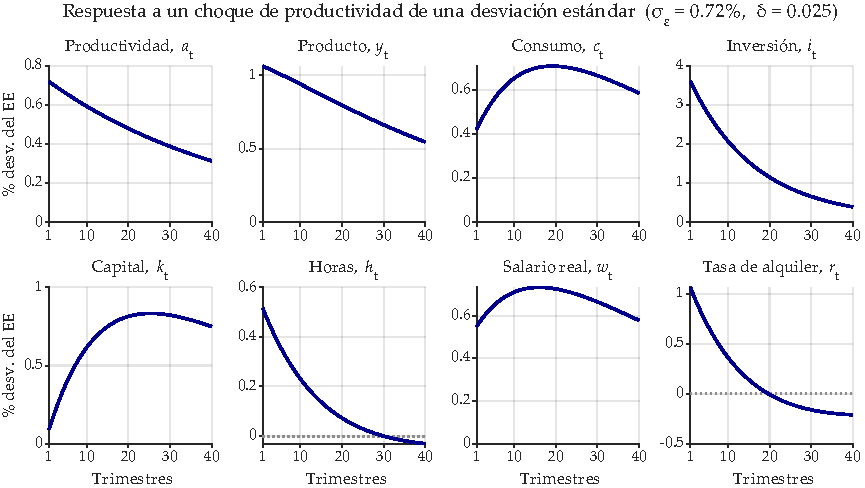
\includegraphics[width=\textwidth]{irf_matlab_base.pdf}
  \par\vspace{0.2cm}\raggedright\small
  Orden sugerido de lectura: $\hat a\to\hat y\to\hat h\to\hat c,\hat\imath\to\hat k\to
  \hat w,\hat r$.
  \fuente{\texttt{oo\_.irfs} de Dynare 7.1, graficadas con \texttt{graficar\_irfs.m}.}
\end{frame}

% S47
\begin{frame}[fragile,label=delta1]{Contraste: depreciación total, $\delta=1$}
  \begin{lstlisting}[language={}]
>> dynare rbc_taller -DDELTA1=1
\end{lstlisting}
  \vspace{0.1cm}
  \centering\small
  \begin{tabular}{@{}lrr@{}}
    \toprule
    \textbf{Impacto, $t=1$ (\%)} & $\delta=0.025$ & $\delta=1$\\
    \midrule
    Producto & 1.064 & 0.720\\
    Consumo & 0.420 & 0.720\\
    Inversión & 3.611 & 0.720\\
    Horas & 0.515 & \num{0}\\
    Persistencia del capital & 0.936 & 0.333\\
    \bottomrule
  \end{tabular}
  \par\vspace{0.3cm}\raggedright\normalsize
  No sobrevive capital: la riqueza es solo el producto de hoy. El hogar consume
  siempre la misma fracción, $c/y=1-\beta(1-\alpha)=0.672$.\par
  \vspace{0.15cm}
  Sin suavizamiento, sustitución e ingreso se cancelan exactamente.
  \fuente{Caso de \textcite{longplosser1983}.}
  \note{Recalibra theta a 3.968. Dynare no guarda oo\_.irfs.h\_eps: la IRF es nula.}
\end{frame}

% S48
\begin{frame}[label=delta1-fig]{Con $\delta=1$, las horas quedan planas}
  \centering
  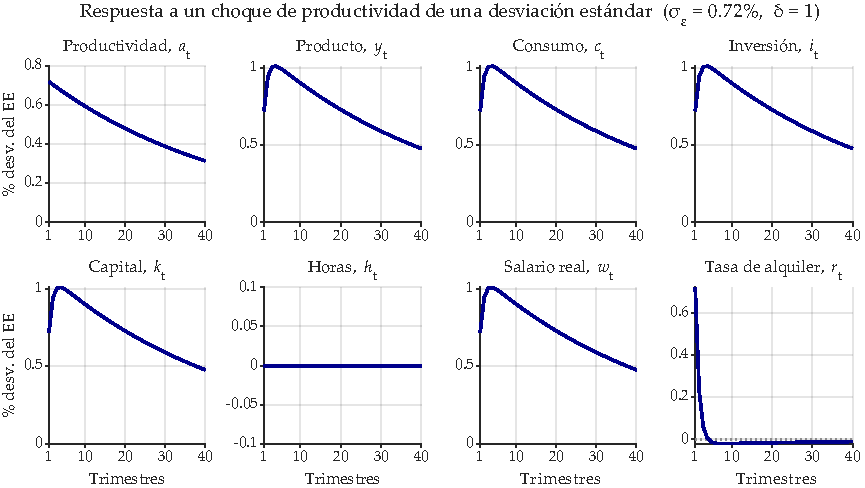
\includegraphics[width=\textwidth]{irf_matlab_delta1.pdf}
  \par\vspace{0.2cm}\raggedright\small
  Producto, consumo, inversión, capital y salario responden \emph{igual} en
  porcentaje: todos son $\hat y_t$, un AR(2) con raíces $\phi$ y $1-\alpha$.
\end{frame}

% S49
\begin{frame}[label=clave]{La ecuación que resume todo}
  Oferta y demanda de trabajo combinadas:
  \[
  \hat y_t-\hat c_t=\frac{\hat h_t}{1-h_{ss}}=1.25\,\hat h_t
  \]
  \begin{center}\large\textbf{Las horas se mueven si y solo si se mueve $c/y$}\end{center}
  \vspace{0.2cm}
  \begin{columns}[T,onlytextwidth]
    \begin{column}{0.48\textwidth}
      \textbf{$\delta=0.025$, $t=1$}\par
      \vspace{0.1cm}
      $1.064-0.420=0.644=1.25\times0.515$\par
      \vspace{0.1cm}
      $c/y$ cae porque el hogar suaviza: las horas suben.
    \end{column}
    \begin{column}{0.48\textwidth}
      \textbf{$\delta=1$, todo $t$}\par
      \vspace{0.1cm}
      $0.720-0.720=0\ \Rightarrow\ \hat h=0$\par
      \vspace{0.1cm}
      $c/y$ es fijo: no hay capital con qué suavizar.
    \end{column}
  \end{columns}
  \par\vspace{0.35cm}
  El capital no solo propaga el choque: es lo que \textbf{activa} la sustitución
  intertemporal del trabajo.
\end{frame}

% S50
\begin{frame}[label=graficos]{De la salida de Dynare a una figura legible}
  \begin{columns}[T,onlytextwidth]
    \begin{column}{0.48\textwidth}
      \centering\textbf{Antes}\par\vspace{0.15cm}
      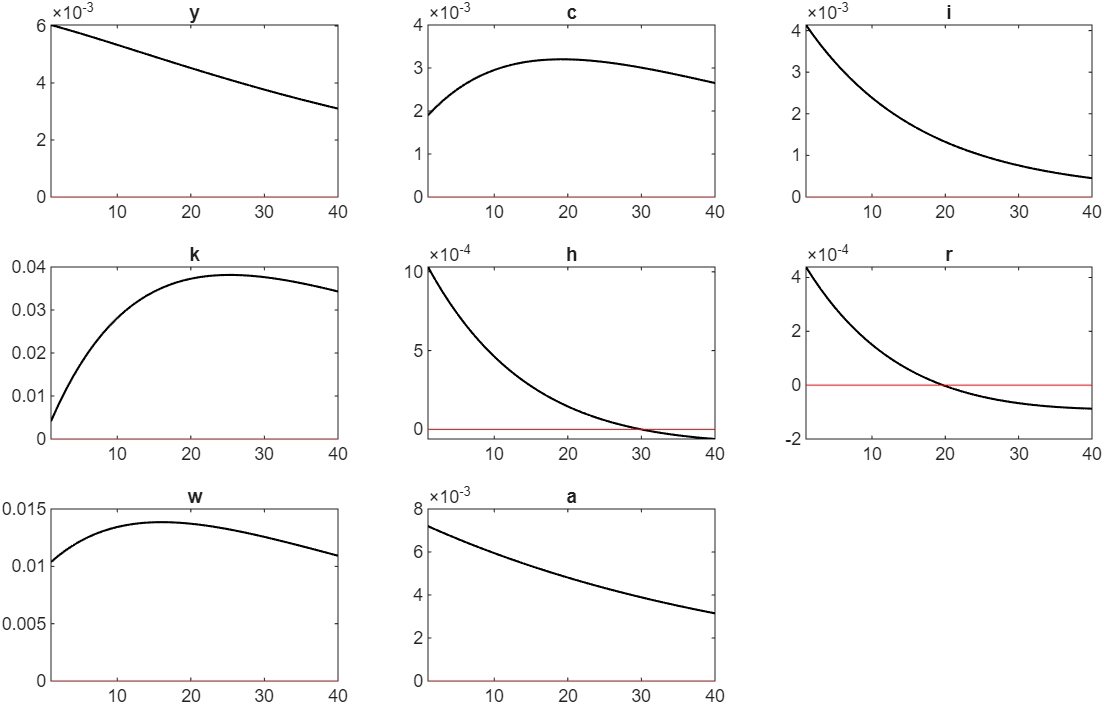
\includegraphics[width=\linewidth]{irf_dynare_default.png}
    \end{column}
    \begin{column}{0.48\textwidth}
      \centering\textbf{Después}\par\vspace{0.15cm}
      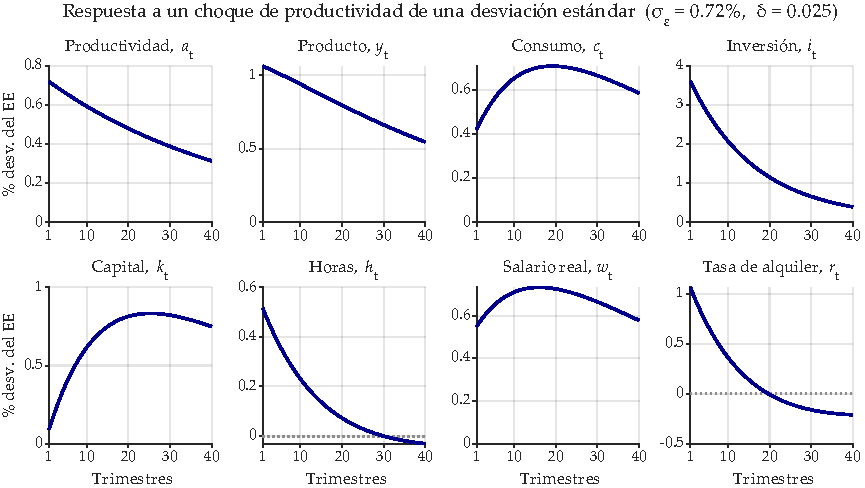
\includegraphics[width=\linewidth]{irf_matlab_base.pdf}
    \end{column}
  \end{columns}
  \par\vspace{0.35cm}\small
  \texttt{graficar\_irfs.m}: una unidad común (\% del EE), títulos con nombre y símbolo,
  ejes que incluyen el cero y tamaño final para imprimir.
  \fuente{Handout, §3.8.3.}
\end{frame}
